\chapter{Analiz'a Teoretic'a}
%\pagestyle{headings}
%
\section{Introducere}
%
%\begin{center}
%\begin{figure}[h]
%    \centering
%    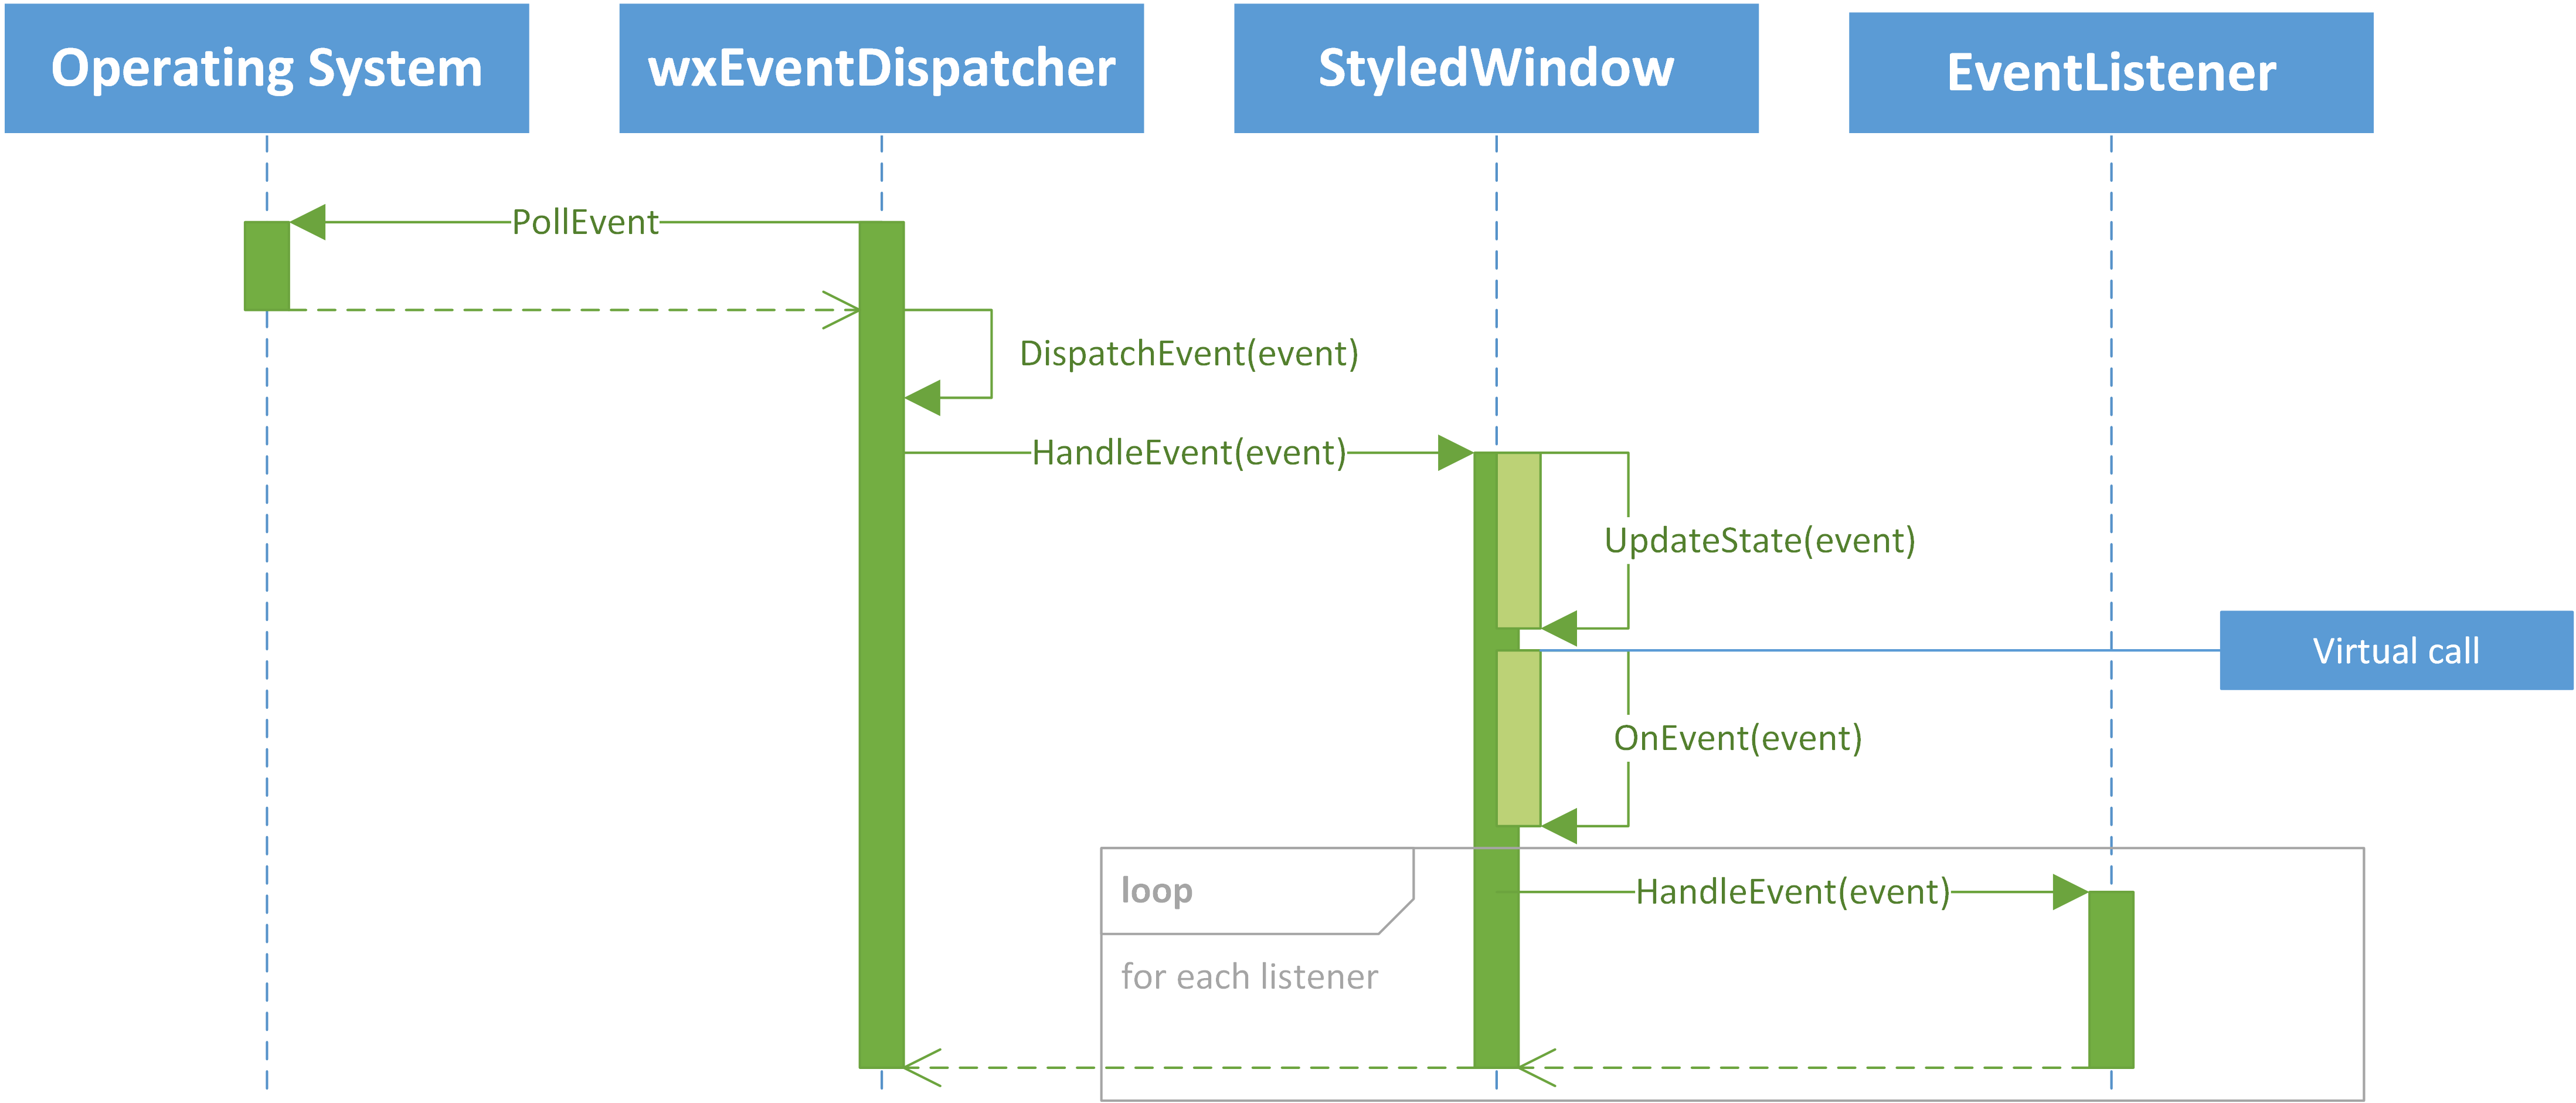
\includegraphics[scale=0.9]{img/ch4_seq_event_processing.png}
%    \label{fig0401}
%    \caption{UML Class Diagram pentru Renderer}
%\end{figure}
%\end{center}
%

Pentru a asigura o bun'a desf'a'surare a activit'a'tii de dezvoltare 'si 'intre'tinere a oric'arui proiect, pentru a asigura flexibilitate la schimb'ari 'in domeniul cerin'telor 'si pentru a preveni hazarduri ulterioare, este necesar'a o analiz'a profund'a 'si am'anun'tit'a a proiectului 'si a componentelor sale 'inainte de 'inceperea implement'arii.

\medskip

Acest capitol 

\begin{itemize}
\item {\bf Cerin'tele proiectului} sunt structurate 'in cazuri de utilizare. 'Incep{\ia}nd cu analiza cerin'telor ne asigur'am ca proiectul atinge ni'ste scopuri bine definite f'ar'a a irosi timp 'in implementarea unor tr'as'aturi nenecesare. 'In plus, putem pleca de la cerin'tele ini'tiale pentru a scrie teste 'si a valida finalizarea proiectului.
\item {\bf Analiza arhitecturilor similare} presupune suprapunerea tehnologiilor deja existente peste cerin'tele proiectului 'si a decide dac'a deciziile luate 'in dezvoltarea altor arhitecturi se aplic'a la acest proiect. 'In cazul 'in care mai multe arhitecturi diferite se prezint'a favorabile, vom decide care este mai potrivit'a.
\item {\bf Prezentarea arhitecturii finale}
\item {\bf Descrierea componentelor}
\end{itemize}

\clearpage

\section{Cazuri de utilizare}

Pentru a modela cerin'tele proiectului, prezent'am urm'atoarele cazuri de utilizare ce au rolul de a documenta cerin'tele func'tionale ale bibliotecii wxStyle.

\begin{figure}[H]
	\centering 
	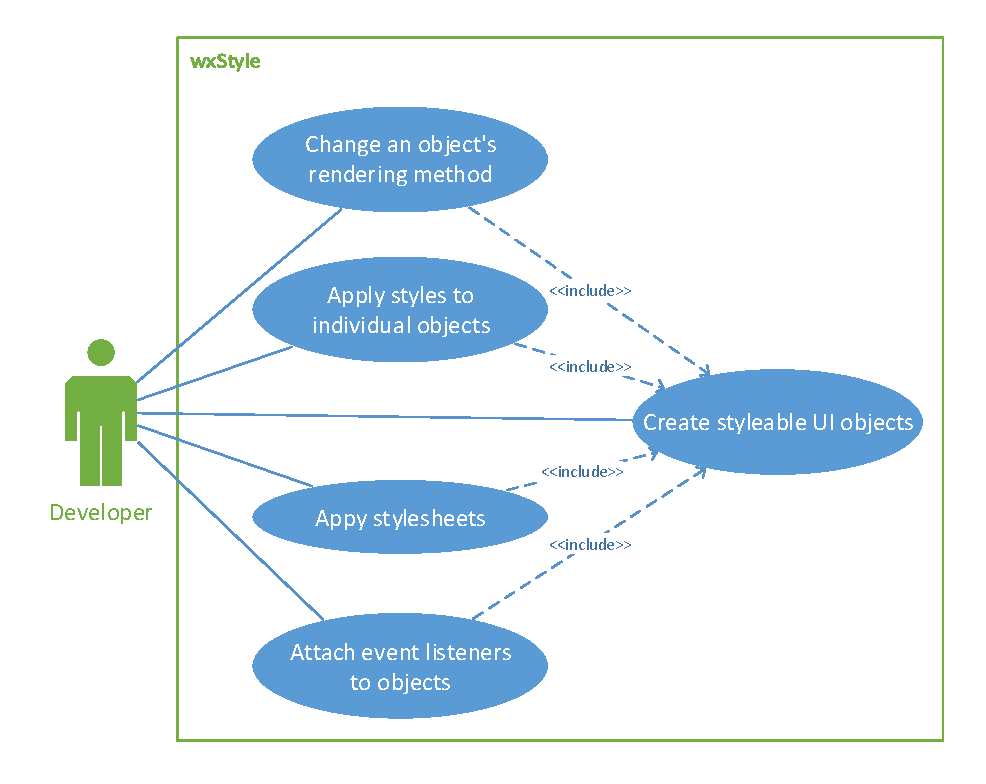
\includegraphics{img/use_case.pdf}
	\label{fig0402}
    \caption{Diagrama UML a cazurilor de utilizare}
\end{figure}

%Cazurile de utilizare prezentate 'in figura \ref{fig0402} acoper'a 

%\clearpage

\subsection{Crearea unui obiect de interfa't'a}
\textbf{Precondi'tie:} Utilizatorul a configurat un mediu de dezvoltare care are acces la bibliotecile wxWidgets 'si wxStyle.
\begin{enumerate}
\item Utilizatorul preg'ate'ste o aplica'tie vizual'a wxWidgets prin implementarea 'si instan'tierea unui wxApp.
\item Utilizatorul declar'a o variabil'a cu unul din tipurile de date ale obiectelor stilizabile 'si 'ii asigneaz'a o instan'ta a acestui tip utiliz{\ia}nd constructorul.
\item Utilizatorul amplaseaz'a obiectul de interfa't'a 'in cadrul unei ferestre, utiliz{\ia}nd constr{\ia}ngeri de amplasare, printr-un proces identic cu amplasarea obiectelor de interfa't'a implementate in biblioteca wxWidgets.
\item Utilizatorul compileaz'a 'si ruleaz'a aplica'tia.
\end{enumerate}
\textbf{Rezultat:} Obiectul de interfa't'a este prezent in cadrul ferestrei.

\subsection{Stilizarea unui obiect de interfa't'a}
\textbf{Precondi'tie:} Parcurgerea cazului de utilizare intitulat \emph{Crearea unui obiect de interfa't'a}.

\begin{enumerate}
\item Utilizatorul construie'ste o instan't'a a clasei \emph{Style} 'si apeleaz'a metodele asociate cu setarea defini'tiilor de stilizare.
\item Utilizatorul ata'seaz'a stilul la un obiect de interfa't'a stilizabil.
\item Utilizatorul compileaz'a 'si ruleaz'a aplica'tia.
\end{enumerate}
\textbf{Rezultat:} Obiectul de interfa't'a este desenat conform defini'tiilor de stil specificate 'in structura de stil.

\subsection{Modificarea procesului de prezentare al unui obiect de interfa't'a}
\textbf{Precondi'tie:} Parcurgerea cazului de utilizare intitulat \emph{Crearea unui obiect de interfa't'a}.
\begin{enumerate}
\item Utilizatorul declar'a o nou'a clasa ce implementeaz'a interfa't'a numit'a \emph{Renderer}.
\item Utilizatorul implementeaz'a metoda \emph{Draw} a acestei clase folosind primitivele de desenare oferite de wxWidgets 'si instruc'tiunile de desenare oferite de wxStyle pentru a desena o reprezentare grafic'a a obiectului de interfa't'a conform st'arii acestuia.
\item Utilizatorul ata'seaz'a o instan't'a a acestei clase unui obiect de interfa't'a stilizabil.
\item Utilizatorul compileaz'a 'si ruleaz'a aplica'tia.
\end{enumerate}
\textbf{Rezultat:} Sistemul prezin'ta obiectul de interfa't'a 'in func'tie de starea sa 'si metoda de desenare implementat'a 'in cadrul clasei de prezentare.

\subsection{Schimbarea aspectului aplica'tiei}
\textbf{Precondi'tie:} Parcurgerea cazului de utilizare intitulat \emph{Crearea unui obiect de interfa't'a}.
\begin{enumerate}
\item Utilizatorul creaz'a op'tional mai multe obiecte de interfa't'a pe care le amplaseaz'a 'in cadrul unei ferestre.
\item Utilizatorul creaz'a o structur'a \emph{Stylesheet}.
\begin{enumerate}
  \item Utilizatorul construie'ste mai multe structuri de tipul \emph{Style} cu scopul de a le asocia unui tip de obiecte de interfa't'a.
  \item Utilizatorul ata'seaz'a stilurile structurii \emph{Stylesheet} 'si le asociaz'a c{\ia}te un nume unic.
  \item Utilizatorul face asocierea dintre tipul obiectului de interfa't'a 'si stilul dorit, ambele identificate prin numele lor, utiliz{\ia}nd metodele de asociere ale structuri \emph{Stylesheet}
\end{enumerate}
\item Utilizatorul aplic'a structura \emph{Stylesheet} prin inregistrarea sa la nivel global.
\end{enumerate}
\textbf{Rezultat:} 'In urma rul'arii aplica'tiei, toate obiectele de interfa't'a stilizabile ce nu au asociate stiluri sau clase de prezentare specificate de utilizator vor fi prezentate conform stilurilor asociate tipului lor din structura \emph{Stylesheet} 'inregistrat'a la nivel global.

\subsection{Procesarea evenimentelor}
\textbf{Precondi'tie:} Parcurgerea cazului de utilizare intitulat \emph{Crearea unui obiect de interfa't'a}.
\begin{enumerate}
\item Utilizatorul identific'a sursa evenimentului, care poate fi eveniment de interac'tiune utilizator sau eveniment generat de un obiect de interfa't'a.
\item Utilizatorul declar'a o nou'a clas'a care extinde interfa't'a de tip \emph{Listener} asociat'a evenimentului.
\item Utilizatorul implementeaz'a acea metod'a care proceseaz'a evenimentul dorit.
\item Utilizatorul ata'seaz'a o instan't'a a acestei clase unuia sau mai multora obiecte de interfa't'a.
\end{enumerate}
\textbf{Rezultat:} Metoda implementa't'a de utilizator este apelat'a 'in momentul producerii unui eveniment de tipul corect.

%\section{Design patterns}
%
%\subsection{Observer}
%
%\subsection{Singleton}
%
%\subsection{Factory}
